\documentclass[9pt]{article}
\usepackage{graphicx} % Required for inserting images
\usepackage{tabularx}
\usepackage{hyperref}
\usepackage{makecell}
\usepackage{makeidx}
\usepackage{eurosym}
\usepackage{fancyhdr}
\usepackage{titlesec}
\usepackage{float}
\newcommand{\firstPage}{
    \thispagestyle{empty}
    \begin{figure}
    \centering
    
\includegraphics[scale=0.7]{Swellfish_logo.png}
    \end{figure}
    \author{
        \date{}
        \href{mailto://swellfish14@gmail.com}{swellfish14@gmail.com} \\
    } 
} 
\usepackage{hyperref}
\usepackage{array}
\usepackage{tabularx}
\usepackage{adjustbox}

\newcounter{verscount}
\setcounter{verscount}{0}
\newcommand{\addversione}[5]{
	\ifdefined\setversione
		\setversione{#1}
	\else\fi
	\stepcounter{verscount}
	\expandafter\newcommand%
		\csname ver\theverscount \endcsname{#1&#2&#3&#4&#5}
}

\newcommand{\listversioni}{
	\ifnum\value{verscount}>1
		\csname ver\theverscount \endcsname
		\addtocounter{verscount}{-1}
		\\\hline
		\listversioni
	\else
		\csname ver\theverscount \endcsname\\\hline
	\fi
}

\newcommand{\makeversioni}{
	\begin{center}
		\begin{tabularx}{\textwidth}{|c|c|X|X|X|}
		\hline
		\textbf{Versione} & \textbf{Data} & \textbf{Redattore} & \textbf{Verificatore} & \textbf{Descrizione} \\
		\hline
		\listversioni
		\end{tabularx}
	\end{center}
	\clearpage
}

\fancypagestyle{genericDocstyle}{
	\pagestyle{fancy}
	\lhead{
\includegraphics[width=1cm]{Swellfish_logo.png}}
	\rhead{Norme di progetto}
}

%\hypersetup{colorlinks=true,urlcolor=blue}

%\newcommand{\tableContent}{

	%{
		%\hypersetup{linkcolor=black}
		%\tableofcontents
	%}
%}
\begin{document}
\graphicspath{ {../templates/img/} }
\setcounter{tocdepth}{4}
\setcounter{secnumdepth}{4}
\title{Piano di progetto}

\firstPage
\maketitle

\begin{center}
	\begin{tabular}{r | l}
		\multicolumn{2}{c}{\textit{Informazioni}}                         \\
		\hline

		\textit{Redattori}    &
		[Davide Porporati, Elena Marchioro, Francesco Naletto]\makecell{} \\

		\textit{Revisori}     &
		[Jude Vensil Barceros]\makecell{}                                 \\
		\textit{Responsabili} &
		[Andrea Veronese]\makecell{}                                      \\
		\textit{Uso}          &
		[Esterno]\makecell{}                                              \\
	\end{tabular}
\end{center}

\begin{center}
	\textbf{Descrizione}\\
	File contenente il piano di progetto per la valutazione dei costi e del raggiungimento delgi obiettivi.
\end{center}

\pagebreak

\printindex
\pagebreak

\tableofcontents
\pagebreak



\addversione{0.0.0}{25/04/2023}{Davide Porporati, Elena Marchioro, Francesco Naletto}{Jude Vensil Barceros}{Creata struttura di base del documento}
\addversione{0.0.1}{27/04/2023}{Davide Porporati, Elena Marchioro, Francesco Naletto}{Jude Vensil Barceros}{Aggiunto diagramma e tabella suddivisione ore}
\addversione{0.0.2}{28/04/2023}{Davide Porporati, Elena Marchioro, Francesco Naletto}{Jude Vensil Barceros}{Aggiunto resoconto primo sprint}
\addversione{0.0.3}{04/05/2023}{Elena Marchioro, Francesco Naletto, Jude Vensil Barceros}{Andrea Veronese}{Aggiunto resoconto secondo sprint e problematiche riscontrate}
\addversione{0.0.4}{11/05/2023}{Francesco Naletto, Jude Vensil Barceros, Andrea Veronese}{Claudio Giaretta}{Aggiunto resoconto terzo sprint}
\addversione{0.0.5}{18/05/2023}{Claudio Giaretta, Jude Vensil Barceros, Andrea Veronese}{Davide Porporati}{Aggiunto resoconto quarto sprint e problematiche}
\addversione{0.0.6}{25/05/2023}{Claudio Giaretta}{Davide Porporati, Elena Marchioro}{Aggiunto resoconto quinto sprint e problematiche}
\addversione{0.0.7}{01/06/2023}{Davide Porporati}{Claudio Giaretta}{Aggiunto resoconto sesto sprint e problematiche}
\addversione{0.0.8}{08/06/2023}{Claudio Giaretta}{Francesco Naletto}{Aggiunto resoconto settimo sprint e problematiche}
\addversione{0.0.9}{07/07/2023}{Claudio Giaretta}{Francesco Naletto}{Aggiunto resoconto ottavo, nono e decimo sprint}
\addversione{0.0.10}{07/07/2023}{Francesco Naletto, Jude Vensil Barceros}{Andrea Veronese}{Aggiunto resoconto undicesimo sprint}
\addversione{0.1.0}{17/07/2023}{Andrea Veronese}{Davide Porporati, Claudio Giaretta}{Verificato documento}
\addversione{1.0.0}{17/07/2023}{Andrea Veronese}{Davide Porporati, Claudio Giaretta}{Aggiornato a versione 1.0.0}
\makeversioni

\section{Introduzione}
Lo scopo di questo documento è quello di fornire un riepilogo del lavoro svolto, del tempo impiegato e dei costi sostenuti, stilato ad intervalli regolari.
Questo documento conterrà una sintesi degli sprint effettuati, con le relative tabelle del costo orario e monetario sostenuto.

\section{Analisi dei rischi}
Nella realizzazione di un prodotto, è fondamentale analizzare, prevedere e gestire i rischi. Per fare ciò, vengono adottate diverse modalità per una corretta interpretazione dei rischi:

\begin{itemize}
	\item \textbf{Identificazione}: si individuano e elencano tutti i possibili rischi che potrebbero verificarsi durante il processo di realizzazione del prodotto.

	\item \textbf{Analisi}: si studia attentamente ogni rischio identificato, valutando le possibili conseguenze che potrebbero derivarne. Questo passaggio aiuta a comprendere meglio la natura dei rischi e a definire le misure da prendere per mitigarli.

	\item \textbf{Piano di contingenza}: viene creato un piano che delinei le azioni da intraprendere nel caso in cui si verifichi uno dei rischi identificati in precedenza. Questo piano serve come guida per affrontare tempestivamente la situazione e minimizzare gli eventuali danni.

	\item \textbf{Controllo}: si utilizzano indicatori o strumenti di monitoraggio per tenere sotto controllo continuo i rischi. Questo permette di rilevare tempestivamente eventuali cambiamenti o nuovi rischi che potrebbero emergere durante il processo di realizzazione del prodotto.
\end{itemize}
Per classificare la probabilità di occorrenza e la pericolosità dei rischi, vengono utilizzate le seguenti sigle:

\begin{itemize}
	\item \textbf{A}: indica una probabilità o una pericolosità alta.
	\item \textbf{M}: indica una probabilità o una pericolosità media.
	\item \textbf{B}: indica una probabilità o una pericolosità bassa.
\end{itemize}

\subsection{Rischi tecnologici}
\begin{center}
	\small
	\begin{tabularx}{\textwidth}{|c|p{3cm}|X|c|c|}
		\hline
		\textbf{Codice} & \textbf{Tipo}            & \textbf{Descrizione}                                                                                                                                                           & \textbf{Prob} & \textbf{Pericolo} \\
		\hline
		RT1             & Inesperienza tecnologica & Questo rischio dipende dal livello di competenza dei membri del team nelle nuove tecnologie e dalla loro capacità di apprendimento.                                            & A             & M                 \\
		\hline
		RT2             & Problemi software        & Questo rischio riguarda eventuali problemi legati al software che i membri del gruppo potrebbero incontrare. Questi problemi potrebbero essere causati da errori del software. & M             & A                 \\
		\hline
	\end{tabularx}
\end{center}
\subsection{Rischi interni}
\begin{center}
	\small
	\begin{tabularx}{\textwidth}{|c|p{3cm}|X|c|c|}
		\hline
		\textbf{Codice} & \textbf{Tipo}       & \textbf{Descrizione}                                                                                                            & \textbf{Prob} & \textbf{Pericolo} \\
		\hline
		RI1             & Impegni personali   & Problemi personali del singolo membro del gruppo che causano ritardi o difficoltà nell'esecuzione dei compiti.                  & M             & B                 \\
		\hline
		RI2             & Discussioni interne & Differenze di approccio e metodo di lavoro tra i vari membri del gruppo che portano a discussioni e rallentamenti nel processo. & M             & B                 \\
		\hline
	\end{tabularx}
\end{center}
\subsection{Rischi organizzativi}
\begin{center}
	\small
	\begin{tabularx}{\textwidth}{|c|p{3cm}|X|c|c|}
		\hline
		\textbf{Codice} & \textbf{Tipo}             & \textbf{Descrizione}                                                                                                        & \textbf{Prob} & \textbf{Pericolo} \\
		\hline
		RO1             & Organizzazione dei lavori & Possibile mancanza di una corretta distribuzione delle attività tra i membri del gruppo, con conseguente disorganizzazione. & B             & M                 \\
		\hline
		RO2             & Risorse sprecate          & Potenziale spreco di risorse in termini di tempo e costi a causa di stime errate.                                           & M             & A                 \\
		\hline
	\end{tabularx}
\end{center}
\subsection{Rischi sui requisiti}
\begin{center}
	\small
	\begin{tabularx}{\textwidth}{|c|p{3cm}|X|c|c|}
		\hline
		\textbf{Codice} & \textbf{Tipo}                   & \textbf{Descrizione}                                                                                        & \textbf{Prob} & \textbf{Pericolo} \\
		\hline
		RR1             & Requisiti incompleti            & Problema causato dalla mancanza di completezza dei requisiti a causa dei cambiamenti nel tempo.             & B             & M                 \\
		\hline
		RR2             & Incomprensione dei requisiti    & Potenziale spreco di risorse in termini di tempo e costi a causa di stime errate.                           & M             & A                 \\
		\hline
		RR3             & Mancato supporto del proponente & Potenziale mancanza di supporto da parte del proponente del prodotto, che potrebbe essere poco disponibile. & B             & B                 \\
		\hline
	\end{tabularx}
\end{center}
\subsection{Piano di contingenza}
\begin{center}
	\small
	\begin{tabularx}{\textwidth}{|c|c|X|}
		\hline
		\textbf{Codice} & \textbf{Pericolo} & \textbf{Piano di contingenza}                                                                                                                                                        \\
		\hline
		RT1             & M                 & Il gruppo si impegna a familiarizzare con le nuove tecnologie necessarie per lo sviluppo del prodotto.                                                                               \\
		\hline
		RT2             & A                 & I membri del gruppo devono avere un dispositivo di backup in caso di guasto hardware, mentre i dati sono salvati in remoto su un repository comune accessibile in qualsiasi momento. \\
		\hline
		RI1             & B                 & In caso di emergenza, il Responsabile riorganizza il lavoro tra i membri del gruppo.                                                                                                 \\
		\hline
		RI2             & B                 & Il Responsabile si impegna a facilitare un accordo tra i membri del gruppo.                                                                                                          \\
		\hline
		RO1             & M                 & Il gruppo discute per suddividere il lavoro in modo equo.                                                                                                                            \\
		\hline
		RO2             & A                 & È necessaria una pianificazione accurata di tempi e costi, e se ciò risulta errato, il Responsabile ridistribuisce il lavoro.                                                        \\
		\hline
		RR1             & M                 & I membri del gruppo si dedicano a un'analisi aggiornata dei requisiti.                                                                                                               \\
		\hline
		RR2             & A                 & Il gruppo pone attenzione alla comprensione dei requisiti e cerca un feedback dal proponente.                                                                                        \\
		\hline
		RR3             & B                 & Il gruppo deve trovare un canale di comunicazione efficace con il proponente.                                                                                                        \\
		\hline
	\end{tabularx}
\end{center}

\section{Pianificazione Generale}
\subsection{Diagramma di Gantt}
Viene qui inserito il diagramma di Gantt, contenente la percentuale di completamento delle varie attività svolte al momento delle redazione.

\floatplacement{figure}{H}
\begin{figure}
	\centering
	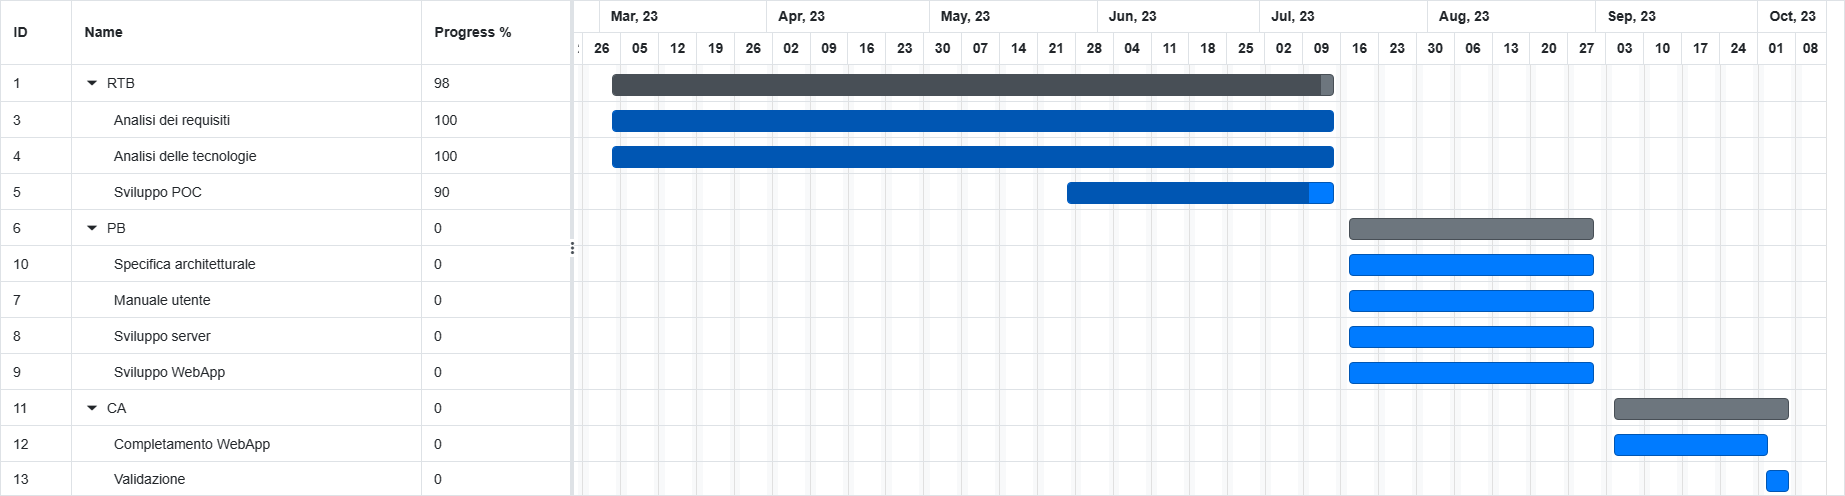
\includegraphics[width=1\textwidth]{img/Gantt.png}
	\caption{Diagramma di Gantt}
\end{figure}


\subsection{Preventivo ore finale}
In questa sezione viene riportato il preventivo orario stimato all'inizio delle attività del progetto. Al termine delle attività verrà valutato se tale preventivo è stato rispettato o meno, fornendo un'analisi dettagliata delle motivazioni che hanno portato all'eventuale superamento delle stime.
\begin{center}
	\begin{tabular}{|l|l|l|l|}
		\hline
		\textbf{Ruolo}  & \textbf{Costo orario} & \textbf{Ore Preventivate} & \textbf{Costo totale} \\
		\hline
		Responsabile    & 30                    & 63                        & 1890\euro             \\
		\hline
		Amministratore  & 20                    & 65                        & 1300\euro             \\
		\hline
		Analista        & 25                    & 88                        & 2200\euro             \\
		\hline
		Progettista     & 25                    & 120                       & 3000\euro             \\
		\hline
		Programmatore   & 15                    & 135                       & 2025\euro             \\
		\hline
		Verificatore    & 15                    & 99                        & 1485\euro             \\
		\hline
		\textbf{Totale} &                       & \textbf{570}              & \textbf{11900\euro}   \\
		\hline
	\end{tabular}
\end{center}

Viene riportata anche la suddivisione delle ore tra i membri preventivata all'inizio delle attività:
\begin{center}
	\begin{tabular}{|l|l|l|l|l|l|l|}
		\hline
		\textbf{Nome}         & \textbf{RS} & \textbf{AM} & \textbf{AL} & \textbf{PG} & \textbf{PT} & \textbf{VR} \\
		\hline
		Andrea Veronese       & 11          & 11          & 16          & 17          & 23          & 17          \\
		\hline
		Claudio Giaretta      & 11          & 11          & 13          & 22          & 23          & 15          \\
		\hline
		Elena Marchioro       & 12          & 10          & 14          & 21          & 22          & 16          \\
		\hline
		Davide Porporati      & 10          & 9           & 16          & 19          & 22          & 19          \\
		\hline
		Francesco Naletto     & 9           & 13          & 14          & 21          & 22          & 16          \\
		\hline
		Jude Vensil Barceros  & 10          & 11          & 15          & 20          & 23          & 16          \\
		\hline
		\textbf{Totale/Ruolo} & 63          & 65          & 88          & 120         & 135         & 99          \\
		\hline
	\end{tabular}
\end{center}
\subsection{Preventivo a finire}
Al termine delle attività verrà effettuata un'analisi mirata a capire le motivazioni che abbiano portato ad uno sforamento delle ore e/o dei costi.
\subsection{Stato d'avanzamento corrente}
Attualmente il gruppo sta concludendo il POC per dimostrare l'efficacia della soluzione proposta e aggiornando la documentazione. Successivamente verrà contattata l'azienda coinvolta per ottenere un feedback valido.

La documentazione viene aggiornata di pari passo con i progressi effettuati, come testimoniato dalle sottoversioni e dalla tabella delle modifiche effettuate.

\section{Metodo di Lavoro}
Il gruppo ha concordato l'utilizzo del framework Scrum come metodo di lavoro agile.
Riportiamo per intero le caratteristiche di ogni "$sprint$":
\begin{itemize}
	\item Durata sprint: una settimana. L'inizo dello sprint è stato concordato al venerdì, mentre il venerdì successivo verrà effettuata una riunone per capire quali obbiettivi siano stati completati e in che metodo.
	\item Ruoli: i ruoli dei membri vengono fatti ruotare settimanalmente, così da garantire un continuo cambiamento di responsabilità.
	\item Obiettivi da completare: vengono decisi prima dell'inizio dello sprint e vengono riportati nella board "$SwellFish$".
\end{itemize}
E' stato previsto che alcuni sprint non vadano a buon fine a causa di difficoltà varie, pertanto non avendo centrato tutti gli obiettivi si valuterà lo stato di avanzamento di quelli iniziati ma non completati.

\section{Sprint Scrum}
\subsection{Sprint 0}
Qui vengono riportate le informazioni relative al primo sprint del gruppo. Questo primo ciclo è caratterizzato dallo svolgimento di attività prettamente documentali e di analisi dei requisiti, pertanto come concordato tra i membri del team i ruoli di analista e programmatore non sono stati impiegati.

Caratteristiche:
\begin{itemize}
	\item Data inizio: 21/04/2023
	\item Data fine preventivata: 28/04/2023
	\item Data fine effettiva: 28/04/2023
\end{itemize}
\subsubsection{Pianificazione}
\begin{center}
	\begin{tabularx}{\textwidth}{|X|X|}
		\hline
		\multicolumn{2}{|c|}{\textbf{Item da realizzare}}  \\
		\hline
		\hline
		\textbf{Item}         & \textbf{Persone richieste} \\
		\hline
		Piano di progetto     & 1                          \\
		\hline
		Piano di qualifica    & 1                          \\
		\hline
		Norme di progetto     & 2                          \\
		\hline
		Analisi dei requisiti & 2                          \\
		\hline
	\end{tabularx}\\[8pt]
	\mbox{}\\
\end{center}
\subsubsection{Preventivo Costi/Ore}
\begin{center}
	\begin{tabularx}{\textwidth}{|X|X|X|X|}
		\hline
		\multicolumn{4}{|c|}{\textbf{Preventivo ore/costi}}                                      \\
		\hline
		\hline
		\textbf{Ruolo}  & \textbf{Costo orario (\euro)} & \textbf{Ore} & \textbf{Prezzo (\euro)} \\
		\hline
		Responsabile    & 30                            & 5            & 150                     \\
		\hline
		Amministratore  & 20                            & 5            & 100                     \\
		\hline
		Analista        & 25                            & 15           & 375                     \\
		\hline
		Progettista     & 25                            & 0            & 0                       \\
		\hline
		Programmatore   & 15                            & 0            & 0                       \\
		\hline
		Verificatore    & 15                            & 4            & 60                      \\
		\hline
		\hline
		\textbf{Totale} &                               & 29           & 685                     \\
		\hline
	\end{tabularx}\\[8pt]
	\mbox{}\\
\end{center}
\subsubsection{Problematiche riscontrate}
Al termine del primo sprint non sono state rilevate particolari problematiche, pertanto questa sezione non ne riporta.
\subsubsection{Resoconto}
\begin{center}
	\begin{tabularx}{\textwidth}{|X|X|X|X|}
		\hline
		\multicolumn{4}{|c|}{\textbf{Preventivo ore/costi}}                                      \\
		\hline
		\hline
		\textbf{Ruolo}  & \textbf{Costo orario (\euro)} & \textbf{Ore} & \textbf{Prezzo (\euro)} \\
		\hline
		Responsabile    & 30                            & 7(+7)        & 210                     \\
		\hline
		Amministratore  & 20                            & 5(+5)        & 100                     \\
		\hline
		Analista        & 25                            & 12(+12)      & 300                     \\
		\hline
		Progettista     & 25                            & 0(+0)        & 0                       \\
		\hline
		Programmatore   & 15                            & 0(+0)        & 0                       \\
		\hline
		Verificatore    & 15                            & 4(+4)        & 60                      \\
		\hline
		\hline
		\textbf{Totale} &                               & 28           & 670                     \\
		\hline
	\end{tabularx}\\[8pt]
	\mbox{}\\
\end{center}


\subsection{Sprint 1}
Qui vengono riportate le informazioni relative al secondo sprint del gruppo. \\
Il secondo ciclo è stato caratterizzato dalla revisione completa delle norme di progetto e dalla revisione degli user case fino ad ora incontrati nell'analisi dei requisiti.\\
Oltre a ciò, è stato realizzato il template da utilizzare per i diari di bordo.


Caratteristiche:
\begin{itemize}
	\item Data inizio: 27/04/2023
	\item Data fine preventivata: 05/05/2023
	\item Data fine effettiva: 04/05/2023
\end{itemize}
\subsubsection{Pianificazione}
\begin{center}
	\begin{tabularx}{\textwidth}{|X|X|}
		\hline
		\multicolumn{2}{|c|}{\textbf{Item da realizzare}}  \\
		\hline
		\hline
		\textbf{Item}         & \textbf{Persone richieste} \\
		\hline
		Piano di progetto     & 1                          \\
		\hline
		Norme di progetto     & 3                          \\
		\hline
		Analisi dei requisiti & 2                          \\
		\hline
	\end{tabularx}\\[8pt]
	\mbox{}\\
\end{center}
\subsubsection{Preventivo Costi/Ore}
\begin{center}
	\begin{tabularx}{\textwidth}{|X|X|X|X|}
		\hline
		\multicolumn{4}{|c|}{\textbf{Preventivo ore/costi}}                                      \\
		\hline
		\hline
		\textbf{Ruolo}  & \textbf{Costo orario (\euro)} & \textbf{Ore} & \textbf{Prezzo (\euro)} \\
		\hline
		Responsabile    & 30                            & 5            & 150                     \\
		\hline
		Amministratore  & 20                            & 4            & 80                      \\
		\hline
		Analista        & 25                            & 9            & 225                     \\
		\hline
		Progettista     & 25                            & 0            & 0                       \\
		\hline
		Programmatore   & 15                            & 0            & 0                       \\
		\hline
		Verificatore    & 15                            & 4            & 60                      \\
		\hline
		\hline
		\textbf{Totale} &                               & 22           & 515                     \\
		\hline
	\end{tabularx}\\[8pt]
	\mbox{}\\
\end{center}
\subsubsection{Problematiche riscontrate}
L'unica problematica riscontrata fino ad ora è stata quella della ristrutturazione delle norme di progetto, pertanto è stato dedicato del tempo aggiuntivo per ristrutturare e incrementare il way of working seguendo il ciclo di vita del software.
L'aggiunta degli UML per gli Use Case è stata rimandata al prossimo sprint per approfondire al meglio il loro funzionamento e perchè lo sprint è durato un giorno in meno a causa della coincidenza con il diario di bordo.
\subsubsection{Resoconto}
\begin{center}
	\begin{tabularx}{\textwidth}{|X|X|X|X|}
		\hline
		\multicolumn{4}{|c|}{\textbf{Preventivo ore/costi}}                                      \\
		\hline
		\hline
		\textbf{Ruolo}  & \textbf{Costo orario (\euro)} & \textbf{Ore} & \textbf{Prezzo (\euro)} \\
		\hline
		Responsabile    & 30                            & 12(+5)       & 150                     \\
		\hline
		Amministratore  & 20                            & 9(+4)        & 80                      \\
		\hline
		Analista        & 25                            & 21(+9)       & 225                     \\
		\hline
		Progettista     & 25                            & 0(+0)        & 0                       \\
		\hline
		Programmatore   & 15                            & 0(+0)        & 0                       \\
		\hline
		Verificatore    & 15                            & 8(+4)        & 60                      \\
		\hline
		\hline
		\textbf{Totale} &                               & 50           & 1185                    \\
		\hline
	\end{tabularx}\\[8pt]
	\mbox{}\\
\end{center}


\subsection{Sprint 2}
Qui vengono riportate le informazioni relative alla terza settimana di sprint del gruppo. \\
Il terzo ciclo è stato caratterizzato dal perfezionamento dell'analisi dei requisiti, individuando nuovi casi d'uso non considerati in precedenza ed espandendoli con la rappresentazione tramite UML.\\



Caratteristiche:
\begin{itemize}
	\item Data inizio: 04/04/2023
	\item Data fine preventivata: 11/05/2023
	\item Data fine effettiva: 11/05/2023
\end{itemize}

\subsubsection{Pianificazione}
\begin{center}
	\begin{tabularx}{\textwidth}{|X|X|}
		\hline
		\multicolumn{2}{|c|}{\textbf{Item da realizzare}}  \\
		\hline
		\hline
		\textbf{Item}         & \textbf{Persone richieste} \\
		\hline
		Piano di progetto     & 1                          \\
		\hline
		Piano di qualifica    & 2                          \\
		\hline
		Analisi dei requisiti & 3                          \\
		\hline
	\end{tabularx}\\[8pt]
	\mbox{}\\
\end{center}
\subsubsection{Preventivo Costi/Ore}
\begin{center}
	\begin{tabularx}{\textwidth}{|X|X|X|X|}
		\hline
		\multicolumn{4}{|c|}{\textbf{Preventivo ore/costi}}                                      \\
		\hline
		\hline
		\textbf{Ruolo}  & \textbf{Costo orario (\euro)} & \textbf{Ore} & \textbf{Prezzo (\euro)} \\
		\hline
		Responsabile    & 30                            & 7            & 210                     \\
		\hline
		Amministratore  & 20                            & 7            & 140                     \\
		\hline
		Analista        & 25                            & 15           & 375                     \\
		\hline
		Progettista     & 25                            & 0            & 0                       \\
		\hline
		Programmatore   & 15                            & 0            & 0                       \\
		\hline
		Verificatore    & 15                            & 5            & 75                      \\
		\hline
		\hline
		\textbf{Totale} &                               & 34           &                         \\ 800\\
		\hline
	\end{tabularx}\\[8pt]
	\mbox{}\\
\end{center}
\subsubsection{Problematiche riscontrate}
Sono sorti dei dubbi riguardanti gli attori nei casi d'uso, pertanto è stata concordata una riunione con Imola Informatica per avere una visione più chiara su questi dubbi.
L'altra problematica riscontrata è inerente alle metriche da utilizzare per valutare la qualità del lavoro.
\subsubsection{Resoconto}
\begin{center}
	\begin{tabularx}{\textwidth}{|X|X|X|X|}
		\hline
		\multicolumn{4}{|c|}{\textbf{Preventivo ore/costi}}                                      \\
		\hline
		\hline
		\textbf{Ruolo}  & \textbf{Costo orario (\euro)} & \textbf{Ore} & \textbf{Prezzo (\euro)} \\
		\hline
		Responsabile    & 30                            & 19(+7)       & 210                     \\
		\hline
		Amministratore  & 20                            & 16(+7)       & 140                     \\
		\hline
		Analista        & 25                            & 36(+15)      & 375                     \\
		\hline
		Progettista     & 25                            & 0(+0)        & 0                       \\
		\hline
		Programmatore   & 15                            & 0(+0)        & 0                       \\
		\hline
		Verificatore    & 15                            & 13(+5)       & 75                      \\
		\hline
		\hline
		\textbf{Totale} &                               & 84           & 1985                    \\
		\hline
	\end{tabularx}\\[8pt]
	\mbox{}\\
\end{center}


\subsection{Sprint 3}
Qui vengono riportate le informazioni relative alla quarta settimana di sprint del gruppo. \\
Il quarto ciclo è stato caratterizzato da una revisione dei casi d'uso dopo aver chiarito i dubbi con una riunione con Imola Informatica e dei relativi UML.\\
E' stata eseguita una valutazione della qualità del progetto seguendo le metriche del piano di qualifica.

Caratteristiche:
\begin{itemize}
	\item Data inizio: 11/04/2023
	\item Data fine preventivata: 18/05/2023
	\item Data fine effettiva: 18/05/2023
\end{itemize}

\subsubsection{Pianificazione}
\begin{center}
	\begin{tabularx}{\textwidth}{|X|X|}
		\hline
		\multicolumn{2}{|c|}{\textbf{Item da realizzare}}               \\
		\hline
		\hline
		\textbf{Item}                      & \textbf{Persone richieste} \\
		\hline
		Piano di progetto                  & 1                          \\
		\hline
		Piano di qualifica                 & 2                          \\
		\hline
		Analisi dei requisiti(inclusi UML) & 3                          \\
		\hline
	\end{tabularx}\\[8pt]
	\mbox{}\\
\end{center}
\subsubsection{Preventivo Costi/Ore}
\begin{center}
	\begin{tabularx}{\textwidth}{|X|X|X|X|}
		\hline
		\multicolumn{4}{|c|}{\textbf{Preventivo ore/costi}}                                      \\
		\hline
		\hline
		\textbf{Ruolo}  & \textbf{Costo orario (\euro)} & \textbf{Ore} & \textbf{Prezzo (\euro)} \\
		\hline
		Responsabile    & 30                            & 3            & 90                      \\
		\hline
		Amministratore  & 20                            & 3            & 60                      \\
		\hline
		Analista        & 25                            & 16           & 400                     \\
		\hline
		Progettista     & 25                            & 0            & 0                       \\
		\hline
		Programmatore   & 15                            & 0            & 0                       \\
		\hline
		Verificatore    & 15                            & 5            & 75                      \\
		\hline
		\hline
		\textbf{Totale} &                               & 27           &                         \\ 625\\
		\hline
	\end{tabularx}\\[8pt]
	\mbox{}\\
\end{center}
\subsubsection{Problematiche riscontrate}
Sono stati rilevati dei dubbi riguardanti gli attori nei casi d'uso e per questo motivo abbiamo effettuato una riunione con Imola Informatica per avere un loro parere.\\
Le altre difficoltà riscontrate riguardano la valutazione delle metriche e i grafici da utilizzare per il piano di qualifica.
\subsubsection{Resoconto}
\begin{center}
	\begin{tabularx}{\textwidth}{|X|X|X|X|}
		\hline
		\multicolumn{4}{|c|}{\textbf{Preventivo ore/costi}}                                      \\
		\hline
		\hline
		\textbf{Ruolo}  & \textbf{Costo orario (\euro)} & \textbf{Ore} & \textbf{Prezzo (\euro)} \\
		\hline
		Responsabile    & 30                            & 22(+3)       & 90                      \\
		\hline
		Amministratore  & 20                            & 19(+3)       & 60                      \\
		\hline
		Analista        & 25                            & 52(+16)      & 400                     \\
		\hline
		Progettista     & 25                            & 0(+0)        & 0                       \\
		\hline
		Programmatore   & 15                            & 0(+0)        & 0                       \\
		\hline
		Verificatore    & 15                            & 18(+5)       & 75                      \\
		\hline
		\hline
		\textbf{Totale} &                               & 111          & 2610                    \\
		\hline
	\end{tabularx}\\[8pt]
	\mbox{}\\
\end{center}

\subsection{Sprint 4}
Qui vengono riportate le informazioni relative alla quinta settimana di sprint del gruppo. \\
Il quinto sprint è stato caratterizzato da una revisione dei casi d'uso dopo e degli uml dopo aver sentito il parere del prof. Cardin.\\
E'stata inoltre redatta l'analisi delle tecnologie in vista dell'inizio della bozza del PoC e l'attività di verifica documentale è proseguita come da programma.


Caratteristiche:
\begin{itemize}
	\item Data inizio: 18/05/2023
	\item Data fine preventivata: 25/05/2023
	\item Data fine effettiva: 25/05/2023
\end{itemize}

\subsubsection{Pianificazione}
\begin{center}
	\begin{tabularx}{\textwidth}{|X|X|}
		\hline
		\multicolumn{2}{|c|}{\textbf{Item da realizzare}}               \\
		\hline
		\hline
		\textbf{Item}                      & \textbf{Persone richieste} \\
		\hline
		Piano di progetto                  & 1                          \\
		\hline
		Analisi dei requisiti(inclusi UML) & 3                          \\
		\hline
		Analisi delle tecnologie           & 2                          \\
		\hline
	\end{tabularx}\\[8pt]
	\mbox{}\\
\end{center}
\subsubsection{Preventivo Costi/Ore}
\begin{center}
	\begin{tabularx}{\textwidth}{|X|X|X|X|}
		\hline
		\multicolumn{4}{|c|}{\textbf{Preventivo ore/costi}}                                      \\
		\hline
		\hline
		\textbf{Ruolo}  & \textbf{Costo orario (\euro)} & \textbf{Ore} & \textbf{Prezzo (\euro)} \\
		\hline
		Responsabile    & 30                            & 2            & 60                      \\
		\hline
		Amministratore  & 20                            & 3            & 60                      \\
		\hline
		Analista        & 25                            & 5            & 125                     \\
		\hline
		Progettista     & 25                            & 5            & 125                     \\
		\hline
		Programmatore   & 15                            & 0            & 0                       \\
		\hline
		Verificatore    & 15                            & 6            & 90                      \\
		\hline
		\hline
		\textbf{Totale} &                               & 21           &                         \\ 460\\
		\hline
	\end{tabularx}\\[8pt]
	\mbox{}\\
\end{center}
\subsubsection{Problematiche riscontrate}
I dubbi riguardanti i casi d'uso e gli uml sono stati discussi e valutati con il docente, pertanto il team si appresta a sistemare le mancanze e le imprecisioni rilevate.
\subsubsection{Resoconto}
\begin{center}
	\begin{tabularx}{\textwidth}{|X|X|X|X|}
		\hline
		\multicolumn{4}{|c|}{\textbf{Preventivo ore/costi}}                                      \\
		\hline
		\hline
		\textbf{Ruolo}  & \textbf{Costo orario (\euro)} & \textbf{Ore} & \textbf{Prezzo (\euro)} \\
		\hline
		Responsabile    & 30                            & 24(+2)       & 60                      \\
		\hline
		Amministratore  & 20                            & 22(+3)       & 60                      \\
		\hline
		Analista        & 25                            & 57(+5)       & 125                     \\
		\hline
		Progettista     & 25                            & 5(+5)        & 125                     \\
		\hline
		Programmatore   & 15                            & 0(+0)        & 0                       \\
		\hline
		Verificatore    & 15                            & 24(+6)       & 90                      \\
		\hline
		\hline
		\textbf{Totale} &                               & 132          & 3070                    \\
		\hline
	\end{tabularx}\\[8pt]
	\mbox{}\\
\end{center}

\subsection{Sprint 5}
Qui vengono riportate le informazioni relative alla sesta settimana di sprint del gruppo. \\
Il sesto ciclo è stato caratterizzato dall'inizio delle attività di progettazione e di sviluppo del POC. \\
Sono stati fatti i mockup per la parte grafica del sito, in modo da avere una baseline da cui partire.


Caratteristiche:
\begin{itemize}
	\item Data inizio: 25/05/2023
	\item Data fine preventivata: 01/06/2023
	\item Data fine effettiva: 01/06/2023
\end{itemize}
\subsubsection{Pianificazione}
\begin{center}
	\begin{tabularx}{\textwidth}{|X|X|}
		\hline
		\multicolumn{2}{|c|}{\textbf{Item da realizzare}}                       \\
		\hline
		\hline
		\textbf{Item}                              & \textbf{Persone richieste} \\
		\hline
		Piano di progetto                          & 1                          \\
		\hline
		Analisi dei requisiti(inclusi UML)         & 1                          \\
		\hline
		POC (incluso frontend, backend e database) & 4                          \\
		\hline
	\end{tabularx}\\[8pt]
	\mbox{}\\
\end{center}
\subsubsection{Preventivo Costi/Ore}
\begin{center}
	\begin{tabularx}{\textwidth}{|X|X|X|X|}
		\hline
		\multicolumn{4}{|c|}{\textbf{Preventivo ore/costi}}                                      \\
		\hline
		\hline
		\textbf{Ruolo}  & \textbf{Costo orario (\euro)} & \textbf{Ore} & \textbf{Prezzo (\euro)} \\
		\hline
		Responsabile    & 30                            & 1            & 30                      \\
		\hline
		Amministratore  & 20                            & 0            & 0                       \\
		\hline
		Analista        & 25                            & 0            & 0                       \\
		\hline
		Progettista     & 25                            & 6            & 150                     \\
		\hline
		Programmatore   & 15                            & 14           & 210                     \\
		\hline
		Verificatore    & 15                            & 3            & 45                      \\
		\hline
		\textbf{Totale} &                               & 24           & 435                     \\
		\hline
	\end{tabularx}\\[8pt]
	\mbox{}\\
\end{center}
\subsubsection{Problematiche riscontrate}
Il monte ore settimanale è in deficit in quanto diversi componenti del gruppo hanno preferito non segnare ore produttive pur avendo fatto autoformazione con il framework utilizzato per lo sviluppo del POC.
\subsubsection{Resoconto}
\begin{center}
	\begin{tabularx}{\textwidth}{|X|X|X|X|}
		\hline
		\multicolumn{4}{|c|}{\textbf{Preventivo ore/costi}}                                      \\
		\hline
		\hline
		\textbf{Ruolo}  & \textbf{Costo orario (\euro)} & \textbf{Ore} & \textbf{Prezzo (\euro)} \\
		\hline
		Responsabile    & 30                            & 25(+1)       & 30                      \\
		\hline
		Amministratore  & 20                            & 22(+0)       & 0                       \\
		\hline
		Analista        & 25                            & 57(+0)       & 0                       \\
		\hline
		Progettista     & 25                            & 11(+6)       & 150                     \\
		\hline
		Programmatore   & 15                            & 14(+14)      & 210                     \\
		\hline
		Verificatore    & 15                            & 27(+3)       & 45                      \\
		\hline
		\hline
		\textbf{Totale} &                               & 156          & 3505                    \\
		\hline
	\end{tabularx}\\[8pt]
	\mbox{}\\
\end{center}

\subsection{Sprint 6}
Qui vengono riportate le informazioni relative alla settima settimana di sprint del gruppo. \\
Il settimo ciclo è stato caratterizzato dalla continuazione dello sviluppo del POC. \\
È stato completato e revisionato il documento "Analisi\_dei\_requisiti", si è inoltre iniziata la parte di sviluppo front-end del POC.


Caratteristiche:
\begin{itemize}
	\item Data inizio: 01/06/2023
	\item Data fine preventivata: 08/06/2023
	\item Data fine effettiva: 08/06/2023
\end{itemize}
\subsubsection{Pianificazione}
\begin{center}
	\begin{tabularx}{\textwidth}{|X|X|}
		\hline
		\multicolumn{2}{|c|}{\textbf{Item da realizzare}}                       \\
		\hline
		\hline
		\textbf{Item}                              & \textbf{Persone richieste} \\
		\hline
		Piano di progetto                          & 1                          \\
		\hline
		Analisi dei requisiti(inclusi UML)         & 1                          \\
		\hline
		POC (incluso frontend, backend e database) & 4                          \\
		\hline
	\end{tabularx}\\[8pt]
	\mbox{}\\
\end{center}
\subsubsection{Preventivo Costi/Ore}
\begin{center}
	\begin{tabularx}{\textwidth}{|X|X|X|X|}
		\hline
		\multicolumn{4}{|c|}{\textbf{Preventivo ore/costi}}                                      \\
		\hline
		\hline
		\textbf{Ruolo}  & \textbf{Costo orario (\euro)} & \textbf{Ore} & \textbf{Prezzo (\euro)} \\
		\hline
		Responsabile    & 30                            & 2            & 60                      \\
		\hline
		Amministratore  & 20                            & 0            & 0                       \\
		\hline
		Analista        & 25                            & 0            & 0                       \\
		\hline
		Progettista     & 25                            & 6            & 150                     \\
		\hline
		Programmatore   & 15                            & 10           & 150                     \\
		\hline
		Verificatore    & 15                            & 3            & 45                      \\
		\hline
		\textbf{Totale} &                               & 24           & 405                     \\
		\hline
	\end{tabularx}\\[8pt]
	\mbox{}\\
\end{center}
\subsubsection{Problematiche riscontrate}
La mancanza di conoscenze delle tecnologie porta via molto tempo all'apprendimento di quest'ultime, il che rallenta lo sviluppo del POC.
\subsubsection{Resoconto}
\begin{center}
	\begin{tabularx}{\textwidth}{|X|X|X|X|}
		\hline
		\multicolumn{4}{|c|}{\textbf{Preventivo ore/costi}}                                      \\
		\hline
		\hline
		\textbf{Ruolo}  & \textbf{Costo orario (\euro)} & \textbf{Ore} & \textbf{Prezzo (\euro)} \\
		\hline
		Responsabile    & 30                            & 28(+3)       & 90                      \\
		\hline
		Amministratore  & 20                            & 22(+0)       & 0                       \\
		\hline
		Analista        & 25                            & 57(+0)       & 0                       \\
		\hline
		Progettista     & 25                            & 17(+6)       & 150                     \\
		\hline
		Programmatore   & 15                            & 22(+8)       & 120                     \\
		\hline
		Verificatore    & 15                            & 31(+4)       & 60                      \\
		\hline
		\hline
		\textbf{Totale} &                               & 177          & 3910                    \\
		\hline
	\end{tabularx}\\[8pt]
	\mbox{}\\
\end{center}

\subsection{Sprint 7}
Qui vengono riportate le informazioni relative alla ottava settimana di sprint del gruppo. \\
In questo ciclo di sprint, il gruppo si è concentrato molto sullo studio delle tecnologie (Nodejs, React) necessarie allo sviluppo del POC. Come preventivato c'è stato un calo di ore lavorate dovuto alla sessione.\\


Caratteristiche:
\begin{itemize}
	\item Data inizio: 08/06/2023
	\item Data fine preventivata: 15/06/2023
	\item Data fine effettiva: 15/06/2023
\end{itemize}
\subsubsection{Pianificazione}
\begin{center}
	\begin{tabularx}{\textwidth}{|X|X|}
		\hline
		\multicolumn{2}{|c|}{\textbf{Item da realizzare}}                       \\
		\hline
		\hline
		\textbf{Item}                              & \textbf{Persone richieste} \\
		\hline
		Piano di progetto                          & 1                          \\
		\hline
		Piano di Qualifica                         & 1                          \\
		\hline
		POC (incluso frontend, backend e database) & 4                          \\
		\hline
	\end{tabularx}\\[8pt]
	\mbox{}\\
\end{center}
\subsubsection{Preventivo Costi/Ore}
\begin{center}
	\begin{tabularx}{\textwidth}{|X|X|X|X|}
		\hline
		\multicolumn{4}{|c|}{\textbf{Preventivo ore/costi}}                                      \\
		\hline
		\hline
		\textbf{Ruolo}  & \textbf{Costo orario (\euro)} & \textbf{Ore} & \textbf{Prezzo (\euro)} \\
		\hline
		Responsabile    & 30                            & 2            & 60                      \\
		\hline
		Amministratore  & 20                            & 2            & 40                      \\
		\hline
		Analista        & 25                            & 0            & 0                       \\
		\hline
		Progettista     & 25                            & 3            & 75                      \\
		\hline
		Programmatore   & 15                            & 8            & 120                     \\
		\hline
		Verificatore    & 15                            & 4            & 60                      \\
		\hline
		\textbf{Totale} &                               & 19           & 355                     \\
		\hline
	\end{tabularx}\\[8pt]
	\mbox{}\\
\end{center}
\subsubsection{Problematiche riscontrate}
Il tempo a disposizione

\subsubsection{Resoconto}
\begin{center}
	\begin{tabularx}{\textwidth}{|X|X|X|X|}
		\hline
		\multicolumn{4}{|c|}{\textbf{Preventivo ore/costi}}                                      \\
		\hline
		\hline
		\textbf{Ruolo}  & \textbf{Costo orario (\euro)} & \textbf{Ore} & \textbf{Prezzo (\euro)} \\
		\hline
		Responsabile    & 30                            & 30(+2)       & 60                      \\
		\hline
		Amministratore  & 20                            & 24(+2)       & 40                      \\
		\hline
		Analista        & 25                            & 57(+0)       & 0                       \\
		\hline
		Progettista     & 25                            & 20(+3)       & 75                      \\
		\hline
		Programmatore   & 15                            & 27(+5)       & 75                      \\
		\hline
		Verificatore    & 15                            & 33(+2)       & 30                      \\
		\hline
		\hline
		\textbf{Totale} &                               & 191          & 4190                    \\
		\hline
	\end{tabularx}\\[8pt]
	\mbox{}\\
\end{center}

\subsection{Sprint 8}
Qui vengono riportate le informazioni relative alla nona settimana di sprint del gruppo. \\
In questo ciclo di sprint il gruppo ha proseguito lo studio delle tecnologie necessarie per il completamento del poc. \\


Caratteristiche:

\begin{itemize}
	\item Data inizio: 15/06/2023
	\item Data fine preventivata: 22/06/2023
	\item Data fine effettiva: 22/06/2023
\end{itemize}
\subsubsection{Pianificazione}
\begin{center}
	\begin{tabularx}{\textwidth}{|X|X|}
		\hline
		\multicolumn{2}{|c|}{\textbf{Item da realizzare}}                       \\
		\hline
		\hline
		\textbf{Item}                              & \textbf{Persone richieste} \\
		\hline
		Piano di progetto                          & 1                          \\
		\hline
		POC (incluso frontend, backend e database) & 5                          \\
		\hline
	\end{tabularx}\\[8pt]
	\mbox{}\\
\end{center}
\subsubsection{Preventivo Costi/Ore}
\begin{center}
	\begin{tabularx}{\textwidth}{|X|X|X|X|}
		\hline
		\multicolumn{4}{|c|}{\textbf{Preventivo ore/costi}}                                      \\
		\hline
		\hline
		\textbf{Ruolo}  & \textbf{Costo orario (\euro)} & \textbf{Ore} & \textbf{Prezzo (\euro)} \\
		\hline
		Responsabile    & 30                            & 2            & 60                      \\
		\hline
		Amministratore  & 20                            & 2            & 40                      \\
		\hline
		Analista        & 25                            & 0            & 0                       \\
		\hline
		Progettista     & 25                            & 2            & 50                      \\
		\hline
		Programmatore   & 15                            & 8            & 120                     \\
		\hline
		Verificatore    & 15                            & 2            & 60                      \\
		\hline
		\textbf{Totale} &                               & 19           & 355                     \\
		\hline
	\end{tabularx}\\[8pt]
	\mbox{}\\
\end{center}
\subsubsection{Problematiche riscontrate}
Il poco tempo a disposizione ha rallentato lo sviluppo del poc.

\subsubsection{Resoconto}
\begin{center}
	\begin{tabularx}{\textwidth}{|X|X|X|X|}
		\hline
		\multicolumn{4}{|c|}{\textbf{Preventivo ore/costi}}                                      \\
		\hline
		\hline
		\textbf{Ruolo}  & \textbf{Costo orario (\euro)} & \textbf{Ore} & \textbf{Prezzo (\euro)} \\
		\hline
		Responsabile    & 30                            & 32(+2)       & 60                      \\
		\hline
		Amministratore  & 20                            & 26(+2)       & 40                      \\
		\hline
		Analista        & 25                            & 57(+0)       & 0                       \\
		\hline
		Progettista     & 25                            & 22(+2)       & 50                      \\
		\hline
		Programmatore   & 15                            & 32(+5)       & 75                      \\
		\hline
		Verificatore    & 15                            & 33(+1)       & 15                      \\
		\hline
		\hline
		\textbf{Totale} &                               & 203          & 4430                    \\
		\hline
	\end{tabularx}\\[8pt]
	\mbox{}\\
\end{center}


\subsection{Sprint 9}
Qui vengono riportate le informazioni relative alla decima settimana di sprint del gruppo. \\
In questo ciclo di sprint il gruppo ha completato la parte front end del poc e ha iniziato a testare le interazioni tra sistema e lampioni \\


Caratteristiche:

\begin{itemize}
	\item Data inizio: 22/06/2023
	\item Data fine preventivata: 29/06/2023
	\item Data fine effettiva: 29/06/2023
\end{itemize}
\subsubsection{Pianificazione}
\begin{center}
	\begin{tabularx}{\textwidth}{|X|X|}
		\hline
		\multicolumn{2}{|c|}{\textbf{Item da realizzare}}     \\
		\hline
		\hline
		\textbf{Item}            & \textbf{Persone richieste} \\
		\hline
		Piano di progetto        & 1                          \\
		\hline
		POC (backend e database) & 4                          \\
		\hline
	\end{tabularx}\\[8pt]
	\mbox{}\\
\end{center}
\subsubsection{Preventivo Costi/Ore}
\begin{center}
	\begin{tabularx}{\textwidth}{|X|X|X|X|}
		\hline
		\multicolumn{4}{|c|}{\textbf{Preventivo ore/costi}}                                      \\
		\hline
		\hline
		\textbf{Ruolo}  & \textbf{Costo orario (\euro)} & \textbf{Ore} & \textbf{Prezzo (\euro)} \\
		\hline
		Responsabile    & 30                            & 2            & 60                      \\
		\hline
		Amministratore  & 20                            & 1            & 20                      \\
		\hline
		Analista        & 25                            & 0            & 0                       \\
		\hline
		Progettista     & 25                            & 4            & 100                     \\
		\hline
		Programmatore   & 15                            & 8            & 120                     \\
		\hline
		Verificatore    & 15                            & 3            & 45                      \\
		\hline
		\textbf{Totale} &                               & 19           & 345                     \\
		\hline
	\end{tabularx}\\[8pt]
	\mbox{}\\
\end{center}
\subsubsection{Problematiche riscontrate}
Difficoltà nell’apprendere l’utilizzo del framework Bulma.io per poter utilizzare in maniera efficace lo sviluppo della parte di CSS e difficoltà interazione tra sistema e API.


\subsubsection{Resoconto}
\begin{center}
	\begin{tabularx}{\textwidth}{|X|X|X|X|}
		\hline
		\multicolumn{4}{|c|}{\textbf{Preventivo ore/costi}}                                      \\
		\hline
		\hline
		\textbf{Ruolo}  & \textbf{Costo orario (\euro)} & \textbf{Ore} & \textbf{Prezzo (\euro)} \\
		\hline
		Responsabile    & 30                            & 34(+2)       & 60                      \\
		\hline
		Amministratore  & 20                            & 27(+1)       & 20                      \\
		\hline
		Analista        & 25                            & 57(+0)       & 0                       \\
		\hline
		Progettista     & 25                            & 26(+4)       & 100                     \\
		\hline
		Programmatore   & 15                            & 41(+9)       & 135                     \\
		\hline
		Verificatore    & 15                            & 36(+3)       & 15                      \\
		\hline
		\hline
		\textbf{Totale} &                               & 221          & 4790                    \\
		\hline
	\end{tabularx}\\[8pt]
	\mbox{}\\
\end{center}

\subsection{Sprint 10}
Qui vengono riportate le informazioni relative all'undicesima settimana di sprint del gruppo. \\
In questo ciclo di sprint il gruppo ha completato la parte di autenticazione dell'applicazione e lo script per la comunicazione dei lampioni \\


Caratteristiche:

\begin{itemize}
	\item Data inizio: 29/06/2023
	\item Data fine preventivata: 07/07/2023
	\item Data fine effettiva: 07/07/2023
\end{itemize}
\subsubsection{Pianificazione}
\begin{center}
	\begin{tabularx}{\textwidth}{|X|X|}
		\hline
		\multicolumn{2}{|c|}{\textbf{Item da realizzare}}     \\
		\hline
		\hline
		\textbf{Item}            & \textbf{Persone richieste} \\
		\hline
		Piano di progetto        & 1                          \\
		\hline
		POC (backend e database) & 4                          \\
		\hline
	\end{tabularx}\\[8pt]
	\mbox{}\\
\end{center}
\subsubsection{Preventivo Costi/Ore}
\begin{center}
	\begin{tabularx}{\textwidth}{|X|X|X|X|}
		\hline
		\multicolumn{4}{|c|}{\textbf{Preventivo ore/costi}}                                      \\
		\hline
		\hline
		\textbf{Ruolo}  & \textbf{Costo orario (\euro)} & \textbf{Ore} & \textbf{Prezzo (\euro)} \\
		\hline
		Responsabile    & 30                            & 3            & 90                      \\
		\hline
		Amministratore  & 20                            & 2            & 40                      \\
		\hline
		Analista        & 25                            & 0            & 0                       \\
		\hline
		Progettista     & 25                            & 2            & 50                      \\
		\hline
		Programmatore   & 15                            & 10           & 150                     \\
		\hline
		Verificatore    & 15                            & 4            & 60                      \\
		\hline
		\textbf{Totale} &                               & 21           & 390                     \\
		\hline
	\end{tabularx}\\[8pt]
	\mbox{}\\
\end{center}
\subsubsection{Problematiche riscontrate}
Difficoltà nell’apprendere l’utilizzo del framework Bulma.io per poter utilizzare in maniera efficace lo sviluppo della parte di CSS e difficoltà interazione tra sistema e API.


\subsubsection{Resoconto}
\begin{center}
	\begin{tabularx}{\textwidth}{|X|X|X|X|}
		\hline
		\multicolumn{4}{|c|}{\textbf{Preventivo ore/costi}}                                      \\
		\hline
		\hline
		\textbf{Ruolo}  & \textbf{Costo orario (\euro)} & \textbf{Ore} & \textbf{Prezzo (\euro)} \\
		\hline
		Responsabile    & 30                            & 37(+3)       & 60                      \\
		\hline
		Amministratore  & 20                            & 29(+2)       & 20                      \\
		\hline
		Analista        & 25                            & 57(+0)       & 0                       \\
		\hline
		Progettista     & 25                            & 28(+2)       & 100                     \\
		\hline
		Programmatore   & 15                            & 50(+9)       & 135                     \\
		\hline
		Verificatore    & 15                            & 39(+3)       & 15                      \\
		\hline
		\hline
		\textbf{Totale} &                               & 240          & 5150                    \\
		\hline
	\end{tabularx}\\[8pt]
	\mbox{}\\
\end{center}

\subsection{Sprint 11}
Qui vengono riportate le informazioni relative alla dodicesima settimana di sprint del gruppo. \\
In questo ciclo di sprint il gruppo ha completato e revisionato la documentazione per la revisione RTB e ha terminato lo sviluppo del POC. \\


Caratteristiche:

\begin{itemize}
	\item Data inizio: 07/07/2023
	\item Data fine preventivata: 14/07/2023
	\item Data fine effettiva: 14/07/2023
\end{itemize}
\subsubsection{Pianificazione}
\begin{center}
	\begin{tabularx}{\textwidth}{|X|X|}
		\hline
		\multicolumn{2}{|c|}{\textbf{Item da realizzare}}     \\
		\hline
		\hline
		\textbf{Item}            & \textbf{Persone richieste} \\
		\hline
		Piano di progetto        & 1                          \\
		\hline
		Piano di qualifica        & 1                          \\
		\hline
		Glossario        & 1                          \\
		\hline
		POC (backend e database) & 2                          \\
		\hline
	\end{tabularx}\\[8pt]
	\mbox{}\\
\end{center}
\subsubsection{Preventivo Costi/Ore}
\begin{center}
	\begin{tabularx}{\textwidth}{|X|X|X|X|}
		\hline
		\multicolumn{4}{|c|}{\textbf{Preventivo ore/costi}}                                      \\
		\hline
		\hline
		\textbf{Ruolo}  & \textbf{Costo orario (\euro)} & \textbf{Ore} & \textbf{Prezzo (\euro)} \\
		\hline
		Responsabile    & 30                            & 3            & 90                      \\
		\hline
		Amministratore  & 20                            & 3            & 60                      \\
		\hline
		Analista        & 25                            & 0            & 0                       \\
		\hline
		Progettista     & 25                            & 10            & 250                      \\
		\hline
		Programmatore   & 15                            & 15           & 225                     \\
		\hline
		Verificatore    & 15                            & 6           & 90                      \\
		\hline
		\textbf{Totale} &                               & 37           & 715                     \\
		\hline
	\end{tabularx}\\[8pt]
	\mbox{}\\
\end{center}
\subsubsection{Problematiche riscontrate}
Nessun particolare dubbio o difficoltà riscontrate


\subsubsection{Resoconto}
\begin{center}
	\begin{tabularx}{\textwidth}{|X|X|X|X|}
		\hline
		\multicolumn{4}{|c|}{\textbf{Preventivo ore/costi}}                                      \\
		\hline
		\hline
		\textbf{Ruolo}  & \textbf{Costo orario (\euro)} & \textbf{Ore} & \textbf{Prezzo (\euro)} \\
		\hline
		Responsabile    & 30                            & 39(+2)       & 60                      \\
		\hline
		Amministratore  & 20                            & 31(+2)       & 40                      \\
		\hline
		Analista        & 25                            & 57(+0)       & 0                       \\
		\hline
		Progettista     & 25                            & 38(+10)       & 250                     \\
		\hline
		Programmatore   & 15                            & 68(+18)       & 270                     \\
		\hline
		Verificatore    & 15                            & 48(+9)       & 135                      \\
		\hline
		\hline
		\textbf{Totale} &                               & 281          & 5905                    \\
		\hline
	\end{tabularx}\\[8pt]
	\mbox{}\\
\end{center}
\end{document}
